\chapter{Asking Millionaire Homeowners How They Got Rich}

This chapter comes from a field interview rather than a board lecture, but the quantitative content is real and worth preserving. We move from spectacle to mechanism: from compounds and gates to compounding, from high income to delayed payoff, from a single store to replicated enterprise, from visible wealth to the hidden arithmetic of debt service, payroll, staffing, and capital formation. The mathematics is therefore modest, but it is not ornamental. Each formula appears only where the transcript itself presses us toward a clear structural idea.

\section{Opening Problem: What Are We Really Looking At?}

The opening is staged with some care. We first see the mansion as an object of astonishment: not merely a large house, but something more like a compound. The host uses that astonishment to create appetite. Then, almost at once, he changes the object. We are no longer looking at wealth for its own sake. We are going to ask how it was built and what advice can be extracted for the younger generation.

The transcript even begins with a small preview of success: a homeowner agrees to answer questions and invites the host inside. Only then does the day settle into its proper frame. Houston is presented, in the host's words, as the number eight city in the world with the most millionaires, and River Oaks becomes the terrain on which the inquiry will be carried out. The method is door-to-door. The constraint is social. One must ask carefully, because rich households are busy, wary, and often protected by gates, distance, or refusal.

\begin{remark}
There are no validated board images for this chapter. Whenever we write an equation or draw a figure, it is a cautious reconstruction of a spoken mechanism, not a transcription from a blackboard.
\end{remark}

The first lesson of the day is therefore methodological before it is financial. Access is scarce. A theory of wealth is not simply found; it must be earned in conversation.

\section{Interview One: Immigration, Relicensing, and the Long Lag to High Income}

The first full answer comes from a physician originally from Pakistan. The speaker immediately gives us a structure that the day will return to again and again: visible wealth does not sit directly on top of visible effort. Between the two there is often a long interval of reconstruction.

She had already been a physician in her home country. After arriving in the United States, she had to repeat licensing examinations and rebuild professional standing. That is the first serious mechanism in the chapter: the endpoint may be impressive, but the path may contain years of delay, duplication, and uncertainty.

Only after that background does the host ask the income question, and only then do we learn that she has made seven figures plus in a single year. The order matters. The transcript refuses to let us read the income figure as effortless glamour. It is presented as the far side of a long restart.

When the host asks for the best financial advice of her life, the lecture makes its first explicit mathematical turn. Her phrasing about the ``wonder of the world'' is garbled, but the point is clear: the power of compounding means that an early dollar does not remain an early dollar.

\subsection{Question \& Answer}

\paragraph{Question.} Why does one dollar saved early matter so much more than one dollar saved late?

\paragraph{Answer.} Because the early dollar is exposed to more rounds of multiplication. If a deposit of amount \(PV\) grows at periodic rate \(r\) for \(n\) periods, then its future value is
\begin{equation}
FV = PV(1+r)^n.
\end{equation}
If instead we make a sequence of equal contributions \(c\), one each period for \(N\) periods, then a minimal reconstruction of the total future value is
\begin{equation}
FV_N = \sum_{k=1}^{N} c(1+r)^{N-k}.
\end{equation}
The transcript gives no numerical rate and no explicit retirement horizon. That is fine. The essential point is the multiplicative asymmetry between early and late deposits.

We can make that asymmetry concrete in the smallest possible worked example. Suppose one contribution \(c\) is made now and an equal contribution \(c\) is made one period later. At a common terminal date,
\begin{align}
FV_{\mathrm{early}} &= c(1+r)^N,\\
FV_{\mathrm{late}}  &= c(1+r)^{N-1}.
\end{align}
Therefore
\begin{equation}
\frac{FV_{\mathrm{early}}}{FV_{\mathrm{late}}} = 1+r.
\end{equation}
So the earlier deposit is larger by a full extra factor of \(1+r\). This is the mathematical content hiding inside the speaker's advice to open the \(401(k)\) the minute one gets a job.

The interview does not end with finance. It turns back to medicine itself. The final answer is that the field is competitive and that standing out required sustained labor: holidays, nights, long stretches of work, and a decade of persistence. The host then walks away and compresses the whole exchange into a short recap: Pakistan, seven figures, compounding. This recap is pedagogically important. It shows us the rule the chapter will follow all day long: anecdote first, mechanism second.

\section{Field Friction: Rejection, Gatekeeping, and the Price of Access}

The chapter now refuses to become too smooth. After a strong first interview, the next several doors do not open. A homeowner declines. Others have no interest. A gated compound cannot talk ``right now.'' This is not filler. It is the price of the method.

If we stripped these moments away, the chapter would read like a curated anthology of millionaire wisdom. The transcript insists on something truer. Access itself is scarce, and the scarcity is instructive. Wealthy operators do not stand around offering complete theories of success. The host must endure indifference, caution, and refusal before another useful answer appears.

This friction also explains a later methodological statement that the host makes explicitly: one must sell oneself in the first five to ten seconds. The threshold problem comes before the theory problem. Before we can ask what scale is, or what debt does, or why compounding matters, we must first be granted a conversation.

So this middle stretch accomplishes two things at once. It preserves the day as an experiment rather than a montage, and it prepares the next major shift. After enough refusals, the host approaches another extraordinary house, repeats the opening language of awe, and is finally invited inside. The narrative rhythm is now clear: gain is intermittent, and that is why each successful answer carries weight.

\section{Interview Two: Franchising, Replication, and Debt Freedom}

The second major interview changes the object of inquiry. With the physician, the question was how an individual profession can culminate in very high income. With the McDonald's operator, the question becomes how a business grows beyond one good location.

The speaker says he has effectively had one job his whole life. He started part-time at McDonald's at seventeen while in college and stayed with the system long enough to build a large portfolio of restaurants. The transcript gives concrete scale:
\begin{equation}
N_{\mathrm{McD}} = 50, \qquad N_{\mathrm{children}} = 19, \qquad N_{\mathrm{family}} = 69.
\end{equation}
This matters because it forces precision on the page. We are not dealing with one well-run restaurant, nor with entrepreneurial charisma in the abstract. We are dealing with repeated units under a common operating framework.

\subsection{Question \& Answer}

\paragraph{Question.} What actually lets a business scale beyond a single successful location?

\paragraph{Answer.} The lecture's answer is franchising, but not as a magic incantation. The claim is that a franchise supplies operating energy because it standardizes a format that can be replicated. The business no longer begins from scratch at every site. Product, process, advertising, and brand recognition arrive partially organized.

A minimal editorial reconstruction is
\begin{equation}
N_{t+1} = N_t + \Delta N_t,
\end{equation}
where \(\Delta N_t > 0\) is feasible only if the operating model is sufficiently repeatable. The point is not to impose a growth theory the transcript never states. It is to preserve the central mechanism: scale appears as increasing unit count under a stable formula.

The logic of the interview may be written in short steps:
\begin{enumerate}
\item Begin with a functioning operating unit.
\item Standardize product and process.
\item Attach the unit to brand recognition and advertising support.
\item Replicate the unit across locations.
\item Supply experience and perseverance, because the franchise does not remove the need for hard work.
\end{enumerate}

The same interview then turns, naturally, from expansion to balance sheet discipline. The operator says he lived on enough money to make ends meet and used the rest to pay down debt. That is a strong financial sequencing rule, and we should preserve it as such. Let \(D_t\) denote total debt at time \(t\), and let
\begin{equation}
R_t = Y_t - E_{\text{needs},t}
\end{equation}
be the residual after minimum living expenditure. Then the debt rule is simply
\begin{equation}
D_{t+1} = D_t - R_t,
\end{equation}
at least while debt remains and \(R_t>0\). The operator emphasizes business debt first, but the broader idea is the same in all cases: freedom increases when fixed claims on future cash decrease.

\begin{figure}
\centering
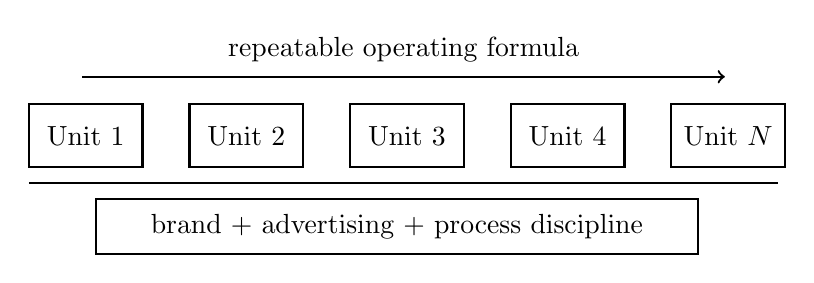
\begin{tikzpicture}[x=1.7cm,y=1cm]
\draw[thick] (0,0) -- (5.6,0);
\foreach \x/\lab in {0/{Unit 1},1.2/{Unit 2},2.4/{Unit 3},3.6/{Unit 4},4.8/{Unit \(N\)}}{
  \draw[thick] (\x,0.2) rectangle (\x+0.85,1.0);
  \node at (\x+0.425,0.6) {\lab};
}
\draw[thick,->] (0.4,1.35) -- (5.2,1.35);
\node at (2.8,1.7) {repeatable operating formula};
\draw[thick] (0.5,-0.9) rectangle (5.0,-0.2);
\node at (2.75,-0.55) {brand + advertising + process discipline};
\end{tikzpicture}
\end{figure}

This schematic is editorial, but it is faithful. Scale is not presented as generalized hustle. It is presented as repeatable organization.

The interview closes with a final warning against impatience. The house did not appear overnight. It was built over time, as part of a family vision, and the speaker wants wealth to be passed on rather than merely displayed. The host then exits in amazement, but he has learned something precise: large visible structures are often downstream from small disciplined repetitions.

\section{Methodological Interlude: First Impressions and the Household Constraint}

Only after the McDonald's interview does the host stop to explain the social mathematics of the entire project. Going up to these homes means asking for time, interrupting someone's day, and creating a decision problem in the first few seconds. One must therefore present oneself quickly and cleanly. This is not a side comment. It is the lecture's own theory of how knowledge was gathered.

That methodological pause leads directly into the next interview. The host approaches another beautiful house, but this time the homeowner is in California and answers remotely. The advice shifts the chapter from expansion to protection. Do not overextend yourself. Live below your means. In bad times, that margin is the difference between safety and strain.

\subsection{Question \& Answer}

\paragraph{Question.} Why is ``living below your means'' more than a moral slogan? Why is it a structural defense?

\paragraph{Answer.} Because the speaker is really describing slack in a cash-flow identity. Let
\begin{equation}
S_t = Y_t - E_t - DS_t,
\end{equation}
where \(Y_t\) is income, \(E_t\) is expenditure, and \(DS_t\) is debt service. Then resilience means
\begin{equation}
S_t > 0.
\end{equation}
If bad times arrive and \(S_t\) is already small, the household remains flexible. If instead
\begin{equation}
S_t < 0,
\end{equation}
then fixed commitments dominate the situation, and trouble is amplified precisely when optionality is most needed.

This is the content of the speaker's advice in its cleanest form:
\begin{equation}
E_t + DS_t < Y_t.
\end{equation}
The host's recap immediately converts the line into operational language: do not over-leverage yourself. Put your head down. Do not look for the easy way out. In the sequence of the day, this is the necessary counterweight to the earlier discussion of growth. The chapter will not let us think about scale without also thinking about survivability.

\begin{figure}
\centering
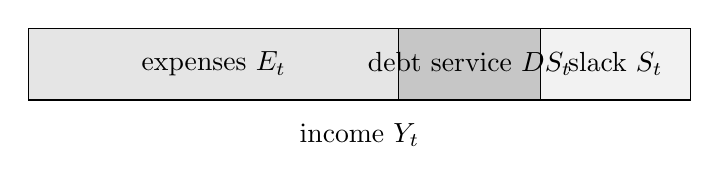
\begin{tikzpicture}[x=1cm,y=1cm]
\draw[thick] (0,0) rectangle (8.4,0.9);
\draw[fill=gray!20] (0,0) rectangle (4.7,0.9);
\draw[fill=gray!45] (4.7,0) rectangle (6.5,0.9);
\draw[fill=gray!10] (6.5,0) rectangle (8.4,0.9);
\node at (2.35,0.45) {expenses \(E_t\)};
\node at (5.6,0.45) {debt service \(DS_t\)};
\node at (7.45,0.45) {slack \(S_t\)};
\node at (4.2,-0.45) {income \(Y_t\)};
\end{tikzpicture}
\end{figure}

\section{Operators, Mentors, and the Burden of Payroll}

The next large house is introduced in the old language of spectacle again, but the content now becomes institutional. The speaker is a former automobile dealer who owned and operated several stores in Houston, later sold his company to AutoNation, and then moved into further investment projects. The host asks the right question here: what do you wish you had known when you started?

The answer is not a slogan. It is a critique of textbook business education. The speaker wishes he had learned more about operational businesses in a form that prepared him for live entrepreneurial reality. One must be mentored. One must be shown what to watch. One does not simply ``read'' the business into existence.

This is then grounded in a turnaround story: a company near bankruptcy is reorganized and becomes the number one Ford truck dealer in the country within roughly a year and a half. The transcript is damaged in places, but the stable line is clear enough. The transformation depended on team organization and on what the speaker calls a rallying point.

The chapter now reaches its largest explicit numbers. Weekly payroll can be
\begin{equation}
B_{\text{week}} \in \{\$150{,}000,\ \$400{,}000,\ \$1{,}000{,}000\}.
\end{equation}
These are not decorative figures. They tell us exactly how the scale of responsibility has changed.

\subsection{Question \& Answer}

\paragraph{Question.} What changes when success is no longer about your own paycheck, but about making payroll for everyone else?

\paragraph{Answer.} The internal structure of the problem changes. Once payroll becomes a large fixed weekly claim, entrepreneurship is no longer merely personal ambition. It becomes the coordination of many livelihoods under one operating burden.

The logic can be laid out in order:
\begin{enumerate}
\item Weekly payroll \(B_{\text{week}}\) is fixed and recurrent.
\item As \(B_{\text{week}}\) grows, more households become dependent on the firm's continuing performance.
\item Leadership can no longer remain private; it must become transmissible across the team.
\item A rallying point is needed to align effort.
\item Outwork still matters, but now it matters through organization rather than through isolated stamina.
\end{enumerate}

The closing counsel in this section is austere and important. One does not need to be the smartest, the biggest, or the fastest. One needs to be the best one can be, and that means outworking everybody else in the organization. We should not literalize this into a numerical decomposition of success. But we should preserve its position in the sequence. The chapter has moved from personal prudence to organizational responsibility, and the resolution is coordinated, sustained work.

\section{Closing Cluster: Staff, Balance, Hidden Cities, and Money as a Tool}

The final movement of the chapter becomes more mosaic-like, but it is not random. A professional musician turned chef says the most important thing in hospitality is staff. Treat staff like gold, and they will treat you like gold. That statement answers the payroll section from the other side. There payroll appeared as burden. Here labor appears as force multiplier. In both cases other people are not incidental to the business. They are constitutive of it.

The chef then adds a balancing clause: work hard, play harder. Do not burn yourself out and let life pass by. The point is not to soften the chapter. It is to keep the objective function honest. Wealth must not consume all experience in the act of producing itself.

The transcript then briefly widens into city drama. A security guard identifies a house as belonging to Tillman Fertitta, owner of the Houston Rockets and Landry's Inc. The host is astonished. That astonishment should stay in the notes, because it serves a genuine conceptual function. Even after a day of door-knocking, the city still contains hidden operators behind ordinary facades of privilege. The curb does not reveal the mechanism.

The last major answer then comes from a Rolls-Royce-owning physician-entrepreneur. He offers the chapter's cleanest late synthesis. First, success in business took about ten years to understand. Second, it does not come easily; one must remain willing to learn. Third, the beginning matters enormously. In the first year after graduation, he says he worked roughly three times as much as a normal doctor in order to save enough capital to secure a bank loan for his first facility.

The minimal reconstruction is
\begin{equation}
\frac{H}{H_{\text{norm}}} \approx 3,
\end{equation}
followed by capital accumulation
\begin{equation}
K_0 = \sum_{t=1}^{T} (Y_t - E_t),
\end{equation}
and then the financing step
\begin{equation}
K_0 \text{ sufficient } \Longrightarrow \text{bank loan } L \text{ for the first facility.}
\end{equation}

This is one of the clearest derivations in the chapter:
\begin{enumerate}
\item Raise labor intensity sharply at the beginning.
\item Convert that labor into unusually high earned income.
\item Hold expenditure down long enough to accumulate capital.
\item Build initial equity \(K_0\).
\item Use that equity to unlock external financing \(L\).
\item Begin the entrepreneurial sequence on a stronger footing.
\end{enumerate}

The final financial advice is then philosophical, but not vague. Do not focus on money as the final object. Think of money as a tool with which one does great things. In mathematical language, money is not the terminal state variable; it is an instrument that changes what projects become feasible. If one mistakes the instrument for the end, then the cars and the houses take over the chapter. The transcript refuses that mistake.

\section{Summary}

The day begins with mansions and ends with mechanisms. In between, the transcript gives us a sequence of operating principles: delayed payoff after migration, compounding through early saving, scale through repeatable systems, freedom through debt reduction, resilience through living below one's means, leadership under payroll pressure, leverage through staff quality, and capital formation through early sacrifice.

What gives the chapter its shape is that it never lets visible wealth stand as its own explanation. Again and again the host extracts the hidden structure from the surface: not the house, but the career path; not the car, but the learning curve; not the portfolio, but the operating system; not the income, but the balance sheet; not the title, but the years of labor behind it.

So the most faithful summary is also the simplest. Wealth, as it appears in this chapter, is rarely a single trick. It is the cumulative effect of time, compounding, disciplined spending, repeated systems, organizational responsibility, and enough sustained work for the arithmetic to turn in one's favor.